 \documentclass{article}
    \usepackage[none]{hyphenat}
    \usepackage{amssymb}
    \usepackage{centernot}
    \usepackage{fixltx2e}
    \usepackage{dsfont}
    \usepackage{upgreek}
    \usepackage{amsmath}
    \usepackage{hhline}
    \usepackage{tipa}
    \usepackage{fancyhdr}
    \usepackage{graphicx}
    \usepackage{setspace}
    \usepackage{hyperref}
    \graphicspath{ {images/} }
    \usepackage{amsmath,amssymb,amsthm, amscd}
\newcommand{\qedend}{\eqno\hfill\rule{1ex}{1ex}}
\renewcommand{\qed}{\hfill\rule{1ex}{1ex}}
\theoremstyle{remark}
\newtheorem*{remark}{Remark}
\onehalfspacing
    \pagestyle{fancy}
    \fancyhead[L]{Report: MLOCR}
    \fancyhead[R]{Chet Aldrich and Laura Biester}
    \begin{document}
	 \section*{MLOCR}
	\label*{Optical Character Recognition using Machine Learning}
	   \subsection*{Introduction}
     Our original goal was the following: given a set of 60,000 handwritten digits, use a machine learning algorithm to make a computer learn how to identify and distinguish between them.

     At first, it was unclear where to start. However, we decided that we could treat the images as an aggregation of many pixels, which were much easier to measure concretely, and then use a machine learning algorithm to identify the number based on these features.

     There were a number of challenges with using this interpretation of the features of an image. First, it doesn't seem intuitive that given a bunch of pixel brightness values, we could determine what number was in the image. Second, it wasn't clear that such a myopic viewpoint would actually lead to accurate results. We could perhaps learn over time what pixel positions are more likely to be used if we are examining a 1, but what happens if we shift the position of the 1? Do the results change?

     Despite the lack of clarity as to whether such features would be realistic, we tried a few machine learning algorithms on the dataset to see if we could produce any meaningful results.
     \subsection*{Implementation}
    	We started by getting data from the MNIST data set and figuring out how to process it. We ended up using a script that turned the MNIST data into a NumPy array, held images and their corresponding labels.

    	Images were stored as 28x28 arrays of information about pixels, which were numbers from 0 to 1. For our project, we considered 0 to be a white pixel and anything above 0 to be a black pixel. From there, we created features based off of the placements of pixels on the screen.

    	We then wrote two machine learning algorithms, Naive Bayes and Perceptron. We ran the data through those two classifiers, and compared their results. These two algorithms, with binary on/off features for each pixel, led to our best results. We allowed users to use only subsets of the training and testing sets to speed up the algorithms, and used randomization to be sure that they were getting a random sample.

    	Over the course of the project, we also explored more classifiers and features. We tried a decision tree, but were not able to achieve above 50\% accuracy using all of the data, which made us feel that it was perhaps not the best classifier for our purposes. We also explored adding a feature to determine if there were any enclosed spaces in the number. However, our algorithm for finding enclosed spaces did not perform the way we has initially expected it to, because we were looking for ``on'' pixels to each side (NSEW) of an ``off'' pixel. We realized that this could be true in almost any number, excluding ones, because of curves. We decided that a more comprehensive feature indicator for determining enclosed spaces would slow down the program too much, so we did not include it in our final implementation.
     \subsection*{Results}
     \begin{table}[h!]
        \centering
        \begin{tabular}{l|l|l}
        Training Quantity & Naive Bayes (with tuning) & Perceptron (with tuning)   \\ \hline
        100               & 75.13\% (253.24 seconds)  & 66.45\% (90.84 seconds)    \\
        500               & 81.57\% (366.62 seconds)  & 80.49\% (141.57 seconds)   \\
        1000              & 82.23\% (354.90 seconds)  & 81.66\% (203.01 seconds)   \\
        5000              & 84.0\% (266.61 seconds)   & 84.10\% (1076.12 seconds)  \\
        10000             & 84.37\% (394.7 seconds)   & 84.64\% (2023.99 seconds)  \\
        20000             & 84.38\% (436.25 seconds)  & 85.44\% (4128.00 seconds)  \\
        30000             & 84.23\% (497.27 seconds)  & 88.62\% (5895.58 seconds)  \\
        40000             & 84.25\% (552.68 seconds)  & 88.26\% (7768.09 seconds)  \\
        50000             & 84.29\% (604.87 seconds)  & 89.14\% (10020.12 seconds) \\
        60000             & 84.31\% (632.77 seconds)  & 89.49\% (11683.14 seconds) \\
        \end{tabular}
     \end{table}

     \begin{figure}[h!]
    \centering
    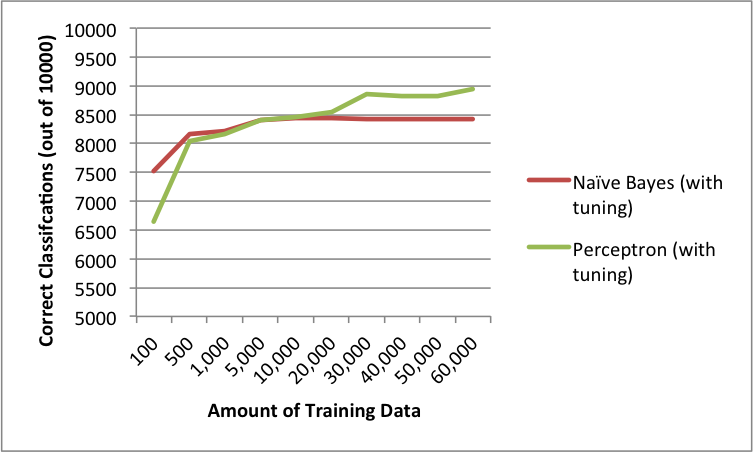
\includegraphics[width=0.8\textwidth]{../graphs/pvsnb.png}
    \caption{Comparing Perceptron and Naive Bayes}
    \label{fig:awesome_image}
    \end{figure}

     We tried a significant number of different training quantities in order to see what was optimal given the training set and time. In terms of total percentage correct, the perceptron led with a slight edge over Naive Bayes with many training examples. However, you'll notice that the Naive Bayes algorithm was much more time efficient to reach a similar level of accuracy. A telling example of this phenomenon are the results with 5000 training instances. Both classifiers reach a similar level of accuracy, but the perceptron took nearly 5 times as long to reach that level of accuracy. In fact, you can see this problem magnifies with larger amounts of training data.

     In our test setting, it was clear that Naive Bayes was much faster given large datasets. However, in many cases we would be allowed to train the classifier prior to using it on data, and this is where the perceptron shines. The classification of test data is very quick with the perceptron, and if we use pretrained values, we can have a more accurate classifier without much of a sacrifice in time other than the initial training time. Running perceptron with pre trained weights only took 26.13 seconds. In this case Naive Bayes loses its edge, taking 191.76 seconds.
     \begin{table}[h!]
     	\centering
    	\begin{tabular}{l|l|l}
    	Training Quantity & Naive Bayes (without tuning) & Naive Bayes (with tuning) \\ \hline
    	100               & 46.56\% (315.31 seconds)     & 75.13\% (253.24 seconds)  \\
    	500               & 58.13\% (316.51 seconds)     & 81.57\% (366.62 seconds)   \\
    	1000              & 61.4\% (327.69 seconds)      & 82.23\% (354.90 seconds)   \\
    	10000             & 79.18\% (330.48 seconds)     & 84.37\% (394.7 seconds)    \\
    	60000             & 83.32\% (476.61 seconds)     & 84.31\% (632.77 seconds)   \\
    	\end{tabular}
     \end{table}
     \begin{table}[h!]
     	\centering
    \begin{tabular}{l|l|l}
    Training Quantity & Perceptron (without tuning) & Perceptron (with tuning)  \\ \hline
    100               & 60.5\% (107.21 seconds)     & 66.45\% (90.84 seconds)    \\
    500               & 80.6\% (120.18 seconds)     & 80.49\% (141.57 seconds)   \\
    1000              & 73.42\% (133.61 seconds)    & 81.66\% (203.01 seconds)   \\
    10000             & 84.22\% (406.90 seconds)    & 84.64\% (2023.99 seconds)  \\
    60000             & 89.15\% (1914.78 seconds)   & 89.49\% (11683.14 seconds) \\
    \end{tabular}\end{table}

    \begin{figure}[h!]
      \centering
      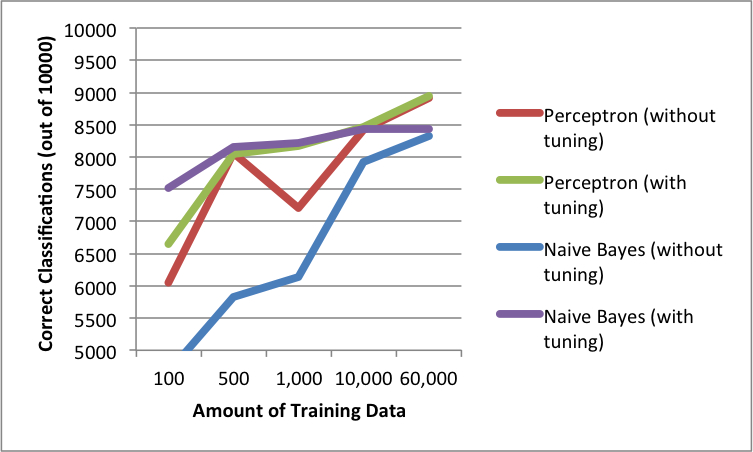
\includegraphics[width=0.8\textwidth]{../graphs/tuning.png}
      \caption{The Effects of Tuning}
    \end{figure}
    \newpage
    Additionally, it became clear during our testing that tuning made classifications of the test data much more accurate given smaller training sets.

    In our case, this seems straightforward. Given less data, accounting for the lack of examples by doing more training or accounting for possibilities that weren't in the training data was helpful for accuracy. However, we noticed that the effects of tuning leveled off considerably as more test examples were included, to the point where it had virtually no effect at all when using 60000 training examples.

    Finally, we looked at common mistakes made by our classifiers. Naives Bayes and Perceptron both commonly mistook 4s for 9s, which could have possibly been prevented by a more rigorous feature for enclosed spaces. It was also interesting that for both classifiers, it was common to make a mistake, for example, classifying an 8 as a 1, but not a 1 as an 8.
\newpage
     \subsection*{Conclusion}
     In the end, we were able to reach an 89.49\% maximum recognition on the test set with a perceptron. This is a relatively high recognition on a fairly complex dataset, which we were surprised to find, especially considering fairly myopic features. However, there is considerable room for improvement.

     We did try determining closed spaces, but it was clear based on the data that the metric was not particularly helpful in increasing the accuracy on the test set. However, there are multiple other possible features we could try, including the longest string of activated (written) pixels in each each row.

     Additionally, we could have tried other classifiers. Early in our trials we attempted a decision tree, which seemed to considerably overfit on our data. Random forests could have alleviated this particular issue.

     With regards to our perceptron, a possible method that we could have used to improve our accuracy on the data would be a neural network.

     In summary, given the techniques we tried we were fairly successful in classifying the MNIST data set.


     \subsection*{Acknowledgements}

     Acknowledgements go to the following groups/individuals responsible for the code and information that was made available to us to complete this project:

     \begin{enumerate}
      \item \href{http://ai.berkeley.edu/project_overview.html}{The Berkeley AI Projects}, for their classification materials that we could look to for general code structure and their util.py file: \\
      \url{http://ai.berkeley.edu/project_overview.html}
      \item \href{http://g.sweyla.com/blog/2012/mnist-numpy/}{Gustav Larsson} for his MNIST data parser: \\
      \url{http://g.sweyla.com/blog/2012/mnist-numpy/}
     \end{enumerate}







    \end{document}
